\documentclass[tikz]{standalone}
\usepackage{tikz}
\usepackage{pgfplots}
\usepackage{pgfmath}
\usepackage{libertine}
\usetikzlibrary{calc}

\renewcommand{\familydefault}{\sfdefault}

\definecolor{mfem@blue}{RGB}{100,150,230}
\definecolor{mfem@green}{RGB}{75,200,75}
\definecolor{mfem@red}{RGB}{200,75,75}
\definecolor{mfem@orange}{RGB}{252,186,3}

\begin{document}

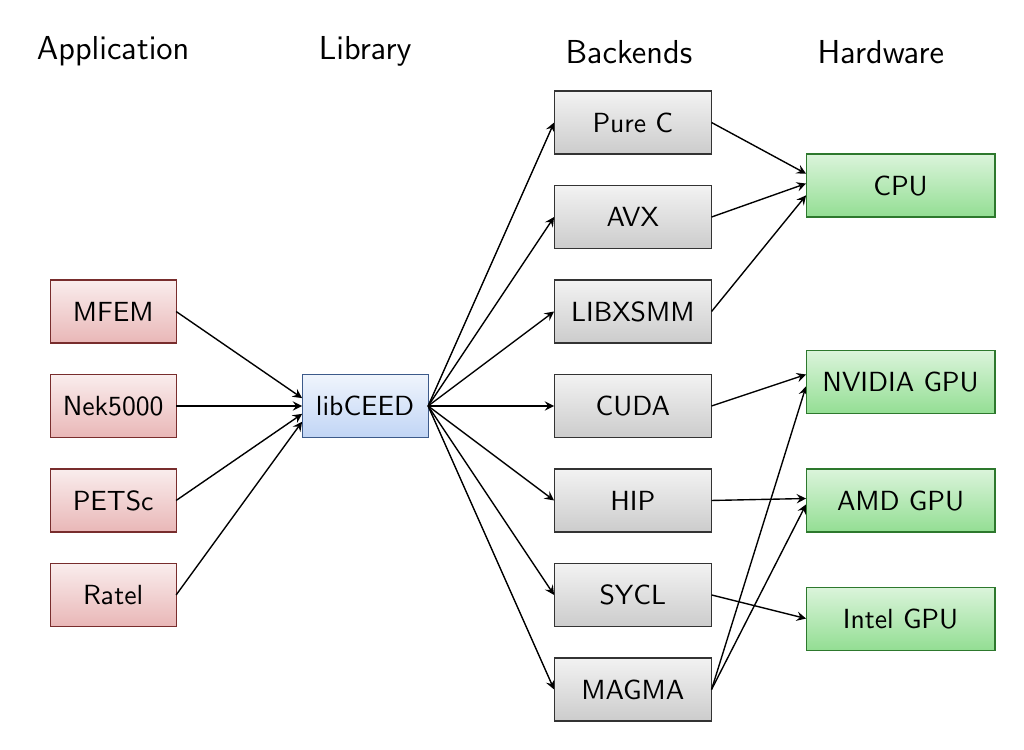
\begin{tikzpicture}

\begin{scope}[shift={(0,-0.6)}]
  \node at (0.8,6.1) {\large Application};

  \draw[
    top color=mfem@red!10!white,
    bottom color=mfem@red!40!white,
    mfem@red!60!black,
  ] (0.0,-1.2) rectangle ++(1.6,0.8)
  node[pos=.5,align=center,color=black] {Ratel};
  \draw[-stealth, line width=0.5pt] (1.6, -0.8) -- ++(1.6,2.4-0.2);

  % PETSc
  \draw[
    top color=mfem@red!10!white,
    bottom color=mfem@red!40!white,
    mfem@red!60!black,
  ] (0.0,0.0) rectangle ++(1.6,0.8)
  node[pos=.5,align=center,color=black] {PETSc};
  \draw[-stealth, line width=0.5pt] (1.6, 0.4) -- ++(1.6,1.2-0.1);

  % Nek5000
  \draw[
    top color=mfem@red!10!white,
    bottom color=mfem@red!40!white,
    mfem@red!60!black,
  ] (0.0,1.2) rectangle ++(1.6,0.8)
  node[pos=.5,align=center,color=black] {Nek5000};
  \draw[-stealth, line width=0.5pt] (1.6, 1.6) -- ++(1.6,0.0);

  % MFEM
  \draw[
    top color=mfem@red!10!white,
    bottom color=mfem@red!40!white,
    mfem@red!60!black,
  ] (0.0,2.4) rectangle ++(1.6,0.8)
  node[pos=.5,align=center,color=black] {MFEM};
  \draw[-stealth, line width=0.5pt] (1.6, 2.8) -- ++(1.6,-1.2+0.1);
\end{scope}

\begin{scope}[shift={(3.2,0)}]
  \begin{scope}[shift={(0,-0.6)}]
  \node at (0.8,6.1) {\large Library};
    \draw[
      top color=mfem@blue!10!white,
      bottom color=mfem@blue!40!white,
      mfem@blue!60!black,
    ] (0.0,1.2) rectangle ++(1.6,0.8)
    node[pos=.5,align=center,color=black] {libCEED};

    \draw[-stealth, line width=0.5pt] (1.6, 1.6) -- ++(1.6,3.6);
    \draw[-stealth, line width=0.5pt] (1.6, 1.6) -- ++(1.6,2.4);
    \draw[-stealth, line width=0.5pt] (1.6, 1.6) -- ++(1.6,1.2);
    \draw[-stealth, line width=0.5pt] (1.6, 1.6) -- ++(1.6,0.0);
    \draw[-stealth, line width=0.5pt] (1.6, 1.6) -- ++(1.6,-1.2);
    \draw[-stealth, line width=0.5pt] (1.6, 1.6) -- ++(1.6,-2.4);
    \draw[-stealth, line width=0.5pt] (1.6, 1.6) -- ++(1.6,-3.6);
  \end{scope}
\end{scope}

\begin{scope}[shift={(6.4,0)}]
  \begin{scope}[shift={(0,-0.6)}]
    \node at (0.95,6.1) {\large Backends};

    % C
    \draw[
      top color=black!5!white,
      bottom color=black!20!white,
      black!80!white,
    ] (0.0,4.8) rectangle ++(2.0,0.8)
    node[pos=.5,align=center,color=black] {Pure C};
    \draw[-stealth, line width=0.5pt] (2.0, 5.2) -- ++(1.2,-0.8+0.15);

    % AVX
    \draw[
      top color=black!5!white,
      bottom color=black!20!white,
      black!80!white,
    ] (0.0,3.6) rectangle ++(2.0,0.8)
    node[pos=.5,align=center,color=black] {AVX};
    \draw[-stealth, line width=0.5pt] (2.0, 4.0) -- ++(1.2,+0.4+0.025);

    % LIBXSMM
    \draw[
      top color=black!5!white,
      bottom color=black!20!white,
      black!80!white,
    ] (0.0,2.4) rectangle ++(2.0,0.8)
    node[pos=.5,align=center,color=black] {LIBXSMM};
    \draw[-stealth, line width=0.5pt] (2.0, 2.8) -- ++(1.2,1.5-0.025);

    \draw[
      top color=black!5!white,
      bottom color=black!20!white,
      black!80!white,
    ] (0.0,1.2) rectangle ++(2.0,0.8)
    node[pos=.5,align=center,color=black] {CUDA};
    \draw[-stealth, line width=0.5pt] (2.0, 1.6) -- ++(1.2,0.4);

    \draw[
      top color=black!5!white,
      bottom color=black!20!white,
      black!80!white,
    ] (0.0,0.0) rectangle ++(2.0,0.8)
    node[pos=.5,align=center,color=black] {HIP};
    \draw[-stealth, line width=0.5pt] (2.0, 0.4) -- ++(1.2,0.0+0.025);

    \draw[
      top color=black!5!white,
      bottom color=black!20!white,
      black!80!white,
    ] (0.0,-1.2) rectangle ++(2.0,0.8)
    node[pos=.5,align=center,color=black] {SYCL};
    \draw[-stealth, line width=0.5pt] (2.0, -0.8) -- ++(1.2,-0.3+0);

    % MAGMA
    \draw[
      top color=black!5!white,
      bottom color=black!20!white,
      black!80!white,
    ] (0.0,-2.4) rectangle ++(2.0,0.8)
    node[pos=.5,align=center,color=black] {MAGMA};
    \draw[-stealth, line width=0.5pt] (2.0, -2.0) -- ++(1.2,4.0-0.15);
    \draw[-stealth, line width=0.5pt] (2.0, -2.0) -- ++(1.2,2.5-0.15);

  \end{scope}
\end{scope}

\begin{scope}[shift={(9.6,0)}]
  \begin{scope}[shift={(0,-0.6)}]
    \node at (0.95,6.1) {\large Hardware};

    % CPU
    \draw[
      top color=mfem@green!20!white,
      bottom color=mfem@green!60!white,
      mfem@green!60!black,
    ] (0.0,4.0) rectangle ++(2.4,0.8)
    node[pos=.5,align=center,color=black] {CPU};

    % CUDA GPU
    \draw[
      top color=mfem@green!20!white,
      bottom color=mfem@green!60!white,
      mfem@green!60!black,
    ] (0.0,1.5) rectangle ++(2.4,0.8)
    node[pos=.5,align=center,color=black] {NVIDIA GPU};

    % ROCm GPU
    \draw[
      top color=mfem@green!20!white,
      bottom color=mfem@green!60!white,
      mfem@green!60!black,
    ] (0.0,-0.0) rectangle ++(2.4,0.8)
    node[pos=.5,align=center,color=black] {AMD GPU};

    \draw[
      top color=mfem@green!20!white,
      bottom color=mfem@green!60!white,
      mfem@green!60!black,
    ] (0.0,-1.5) rectangle ++(2.4,0.8)
    node[pos=.5,align=center,color=black] {Intel GPU};

  \end{scope}
\end{scope}

\end{tikzpicture}
\end{document}
